%!TEX root = ../dissertation.tex

\chapter{Evaluation}
\label{chapter:evaluation}
% Introduce evaluation...
% Main goals
% Setup used

After the implementation of this solution, explained in chapter \ref{chapter:implementation}, some experiments were performed in order to test it.
The Restaurant and Smart Museum apps, described in section \ref{sec:solution_examples} were used in these experiments. In both, the app tries to scan for the nearest beacon, which means, somehow, it has into account the distance from the beacons. The \gls{API} used to handle the beacons has a method to get the distance from a given beacon.
We need to check if is trustworthy the distance's value we get from the beacons \gls{API}.

The app for end users, described in section \ref{sec:solution_mobile_app_for_users}, needs to run, in background, in order to let the user be notified when he/she is nearby any Smart Place, instead of require his/her interaction. However, as any service running in background, that can have a negative impact on the mobile device's resources usage, such as, \gls{CPU}, memory, network, etc.
A set of experiments was performed to evaluate the overhead introduced by our solution and if it is acceptable, having an app, running in background, scanning for beacons.

A Motorola\texttrademark
Moto G\footnote{http://www.gsmarena.com/motorola\_moto\_g-5831.php} smartphone was used to run the mobile application. This device has the following specifications:
\begin{description}
  \item[\gls{CPU}:] Quad-core 1.2 GHz Cortex-A7\footnote{http://www.arm.com/products/processors/cortex-a/cortex-a7.php}
  \item[\gls{GPU}:] Adreno 305
  \item[\gls{RAM}:] 1 \gls{GB}
  \item[Internal storage:]: 16 \gls{GB}
  \item[Screen:] 4.5 inches
  \item[Battery:] Non-removable Li-Ion 2070 \gls{mAh} battery
  \item[\gls{OS}:] Android 5.0.2 (Lollipop\footnote{https://www.android.com/versions/lollipop-5-0})
\end{description}

\section{Methodology}
\label{sec:methodology}
% Previous two problems raised
% Two kinds of experiments
% Tables outlining the experiments
Previously, two problems were raised. First, our solution relies on the beacons \gls{API} to get the nearest beacon. Second, having the mobile app for end users scanning for beacons peridically can imply some overhead in terms of mobile device's resources usage, such as, \gls{CPU}, memory, network connection, etc.
Two experiments were made in order to evaluate the impact of these two problems.

The first set of experiments, summarized in Table~\ref{tab:experiments_nearest_beacon}, try to test if the mobile app can detect the nearest beacon.
In these experiments, the Smart Musem example was used.
In each experiment, it ran for 5 minutes. Then, in Android Studio log output, it was possible to check how many times each beacon was detected as the nearest one.

\begin{table}[]
\centering
\begin{tabular}{@{}|l|c|c|c|c|@{}}
\toprule
\multicolumn{1}{|c|}{}                & \multicolumn{4}{c|}{{\bf Experiments}}                                                                            \\ \midrule
\multicolumn{1}{|c|}{{\bf Variables}} & {\bf 1}                     & {\bf 2}                   & {\bf 3}                     & {\bf 4}                   \\ \midrule
Events                                & \multicolumn{4}{c|}{\begin{tabular}[c]{@{}c@{}}For each beacon, \\ how many times \\ it was scanned\end{tabular}} \\ \midrule
Number of beacons                     & \multicolumn{4}{c|}{3}                                                                                            \\ \midrule
Interval between each scan (seconds)  & \multicolumn{4}{c|}{10}                                                                                           \\ \midrule
Experiment duration (minutes)         & \multicolumn{4}{c|}{5}                                                                                            \\ \midrule
Distance between beacons (meters)     & \multicolumn{1}{r|}{0.5}    & \multicolumn{1}{r|}{1}    & \multicolumn{1}{r|}{1.5}    & \multicolumn{1}{r|}{2}    \\ \bottomrule
\end{tabular}
\caption[Nearest beacon experiments summary]{Experiments to get the accuracy of the method to get the nearest beacon}
\label{tab:experiments_nearest_beacon}
\end{table}


The smartphone and the three beacons were disposed in a layout, where each beacon was equally distant from each other and the smartphone was close to one of them, as shown in Figure~\ref{fig:experiments_nearest_beacon}, where value d, is the distance between beacons and s is the distance between the smartphone and the first beacon. The names below each beacon (ice, blueberry and mint), were provided by Estimote in the developer pack.

In this first set of experiments, the value d starts at 50 centimeters and is increased by 50 centimeters in each experiment until the 4th one where d is 2 meters.

\begin{figure}[!ht]
  \centering
    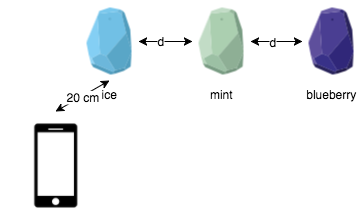
\includegraphics[width=0.5\textwidth, keepaspectratio]{images/nearest_beacon}
    \caption{Beacons with equal distance from each other}
    \label{fig:experiments_nearest_beacon}
\end{figure}

The second set of experiments, aims to get a good insight about the overhead introduced by the mobile app that runs on background and scans for beacons periodically. Table~\ref{tab:experiments_resources} summarizes them. It was also used the same layout as in the previous set of experiments. In the first half experiments, \gls{WiFi} connection was used and in the remaining ones, \gls{3G} connection was used. These two types of data connection are different, in terms of bandwith, speed, etc. Using these two different connections allowed us to understand if the resources usage is acceptable even if no \gls{WiFi} connection is available. Using Android Studio Device Monitor tool\footnote{http://developer.android.com/tools/help/monitor.html} we were able to collect metrics such as, \gls{CPU} usage [????], memory consumption, data network traffic (received and transmitted) and latency of each request.
Different intervals between each scan were tested to see the impact of its value in the mobile device's resources usage.
During each experiment, at each three and half minutes, the first beacon (ice) exchanged place with the second (blueberry). Then, after three and half minutes again, blueberry beacon exchanged place with the third one (mint). The total experiment duration was ten and half minutes. The idea of these exchanges was to simulate the user walking through the all three beacons in a given place.

% Please add the following required packages to your document preamble:
% \usepackage{booktabs}
% \usepackage{graphicx}
\begin{table}[]
\centering
\begin{tabular}{@{}|l|c|c|c|c|c|c|@{}}
\toprule
                                     & \multicolumn{6}{c|}{{\bf Experiments}}                                                                                                                      \\ \midrule
{\bf Variables}                      & {\bf 1}                 & {\bf 2}                 & {\bf 3}                  & {\bf 4}                 & {\bf 5}                 & {\bf 6}                  \\ \midrule
Data connection type                 & \multicolumn{3}{c|}{WiFi}                                                    & \multicolumn{3}{c|}{3G}                                                      \\ \midrule
Metrics                              & \multicolumn{6}{c|}{\begin{tabular}[c]{@{}c@{}}CPU usage, memory usage, \\ data network traffic and latency\end{tabular}}                                   \\ \midrule
Number of beacons                    & \multicolumn{6}{c|}{3}                                                                                                                                      \\ \midrule
Interval between each scan (seconds) & \multicolumn{1}{r|}{10} & \multicolumn{1}{r|}{60} & \multicolumn{1}{r|}{300} & \multicolumn{1}{r|}{10} & \multicolumn{1}{r|}{60} & \multicolumn{1}{r|}{300} \\ \midrule
Experiment duration (minutes)        & \multicolumn{6}{c|}{10.5}                                                                                                                                   \\ \midrule
Distance between beacons (meters)    & \multicolumn{6}{c|}{2}                                                                                                                                      \\ \bottomrule
\end{tabular}
\caption{Experiments to evaluate the mobile device's resources usage}
\label{tab:experiments_resources}
\end{table}


\section{Results}
\label{sec:results}
